%File: main.tex
%Based on formatting-instructions.tex, distributed as part of the aaai submission information.
\documentclass[letterpaper]{article}
\usepackage{aaai}
\usepackage{times}
\usepackage{helvet}
\usepackage{courier}
\frenchspacing

% Package and images path
\usepackage{graphicx}
\graphicspath{ {images/} }

\setlength{\pdfpagewidth}{8.5in}
\setlength{\pdfpageheight}{11in}
\pdfinfo{
/Title (Link Prediction in FanFiction Networks: Early Work Toward Collaborative Filtering)
/Author (Alexander Hayes)}
\setcounter{secnumdepth}{0}

\begin{document}
% The file aaai.sty is the style file for AAAI Press
% proceedings, working notes, and technical reports.
%

\title{Link Prediction in FanFiction Networks:\\Early Work Toward Collaborative Filtering}
\author{Alexander L. Hayes\\
The University of Texas at Dallas\\
alexander.hayes@utdallas.edu\\
}

\maketitle
\begin{abstract}
\begin{quote}
The author performs link prediction on metadata and social network data scraped from FanFiction.Net (the world's largest repository of user-submitted fanfiction), applying statistical relational learning to predict authorship of a story through two tree-based models: relational dependency networks (RDNs) learned via gradient boosting, and RDNs learned via gradient boosting with soft-margin constraints set on the cost of false positives and false negatives. Results are shown for four types of fanfiction, and transfer is applied to show how structure learning generalizes across different social networks. Code and documentation for the experiments are available in the Appendix section of this paper and on GitHub.\footnote{\texttt{https://github.com/batflyer/FanFiction-\\Collaborative-Filtering}}
\end{quote}
\end{abstract}

\section{Introduction}
A ``fanfic'' is a creative work where a person adapts or extends an existing work of fiction.  An author may write a completely different ending to the source material, he or she may tell a similar story but insert several characters of their own creation, or he or she may cut the characters from one story and place them in a completely different environment.  What if the characters from Tolkien's \textit{The Lord of the Rings} were in a modern-day high school?  What if Jean-Luc Picard landed the USS Enterprise on \textit{Avatar}'s Pandora?  What if \textit{Phantom of the Opera} had a completely different ending?

Scenarios such as these are played out on places such as FanFiction.Net, where authors and community members write, read, and review one another's stories across thousands of possible fandoms.  The practice of writing and sharing fanfiction is sometimes compared to oral-traditional storytelling; rather than media being produced and distributed by a few popular people or publishing groups: stories are shared, retold, and adapted between a community of people; building universes and mythos around stories.

FanFiction has been observed through a variety of academic lenses; such as psychology, sociology, and (more recently) computer science. Though many have taken interest in the subject, a common viewpoint is that fanfiction is poorly understood within academic literature, or that previous attempts to analyze fanfiction communities have been performed in disruptive manners \cite{larsen2011fandom}. \cite{barnes2015fanfiction} noted that the subject at the time of writing had almost entirely been understood from a qualitative standpoint, but posed several questions which may be answered in part by large-scale quantitative analysis.

\begin{figure}
    \centering
    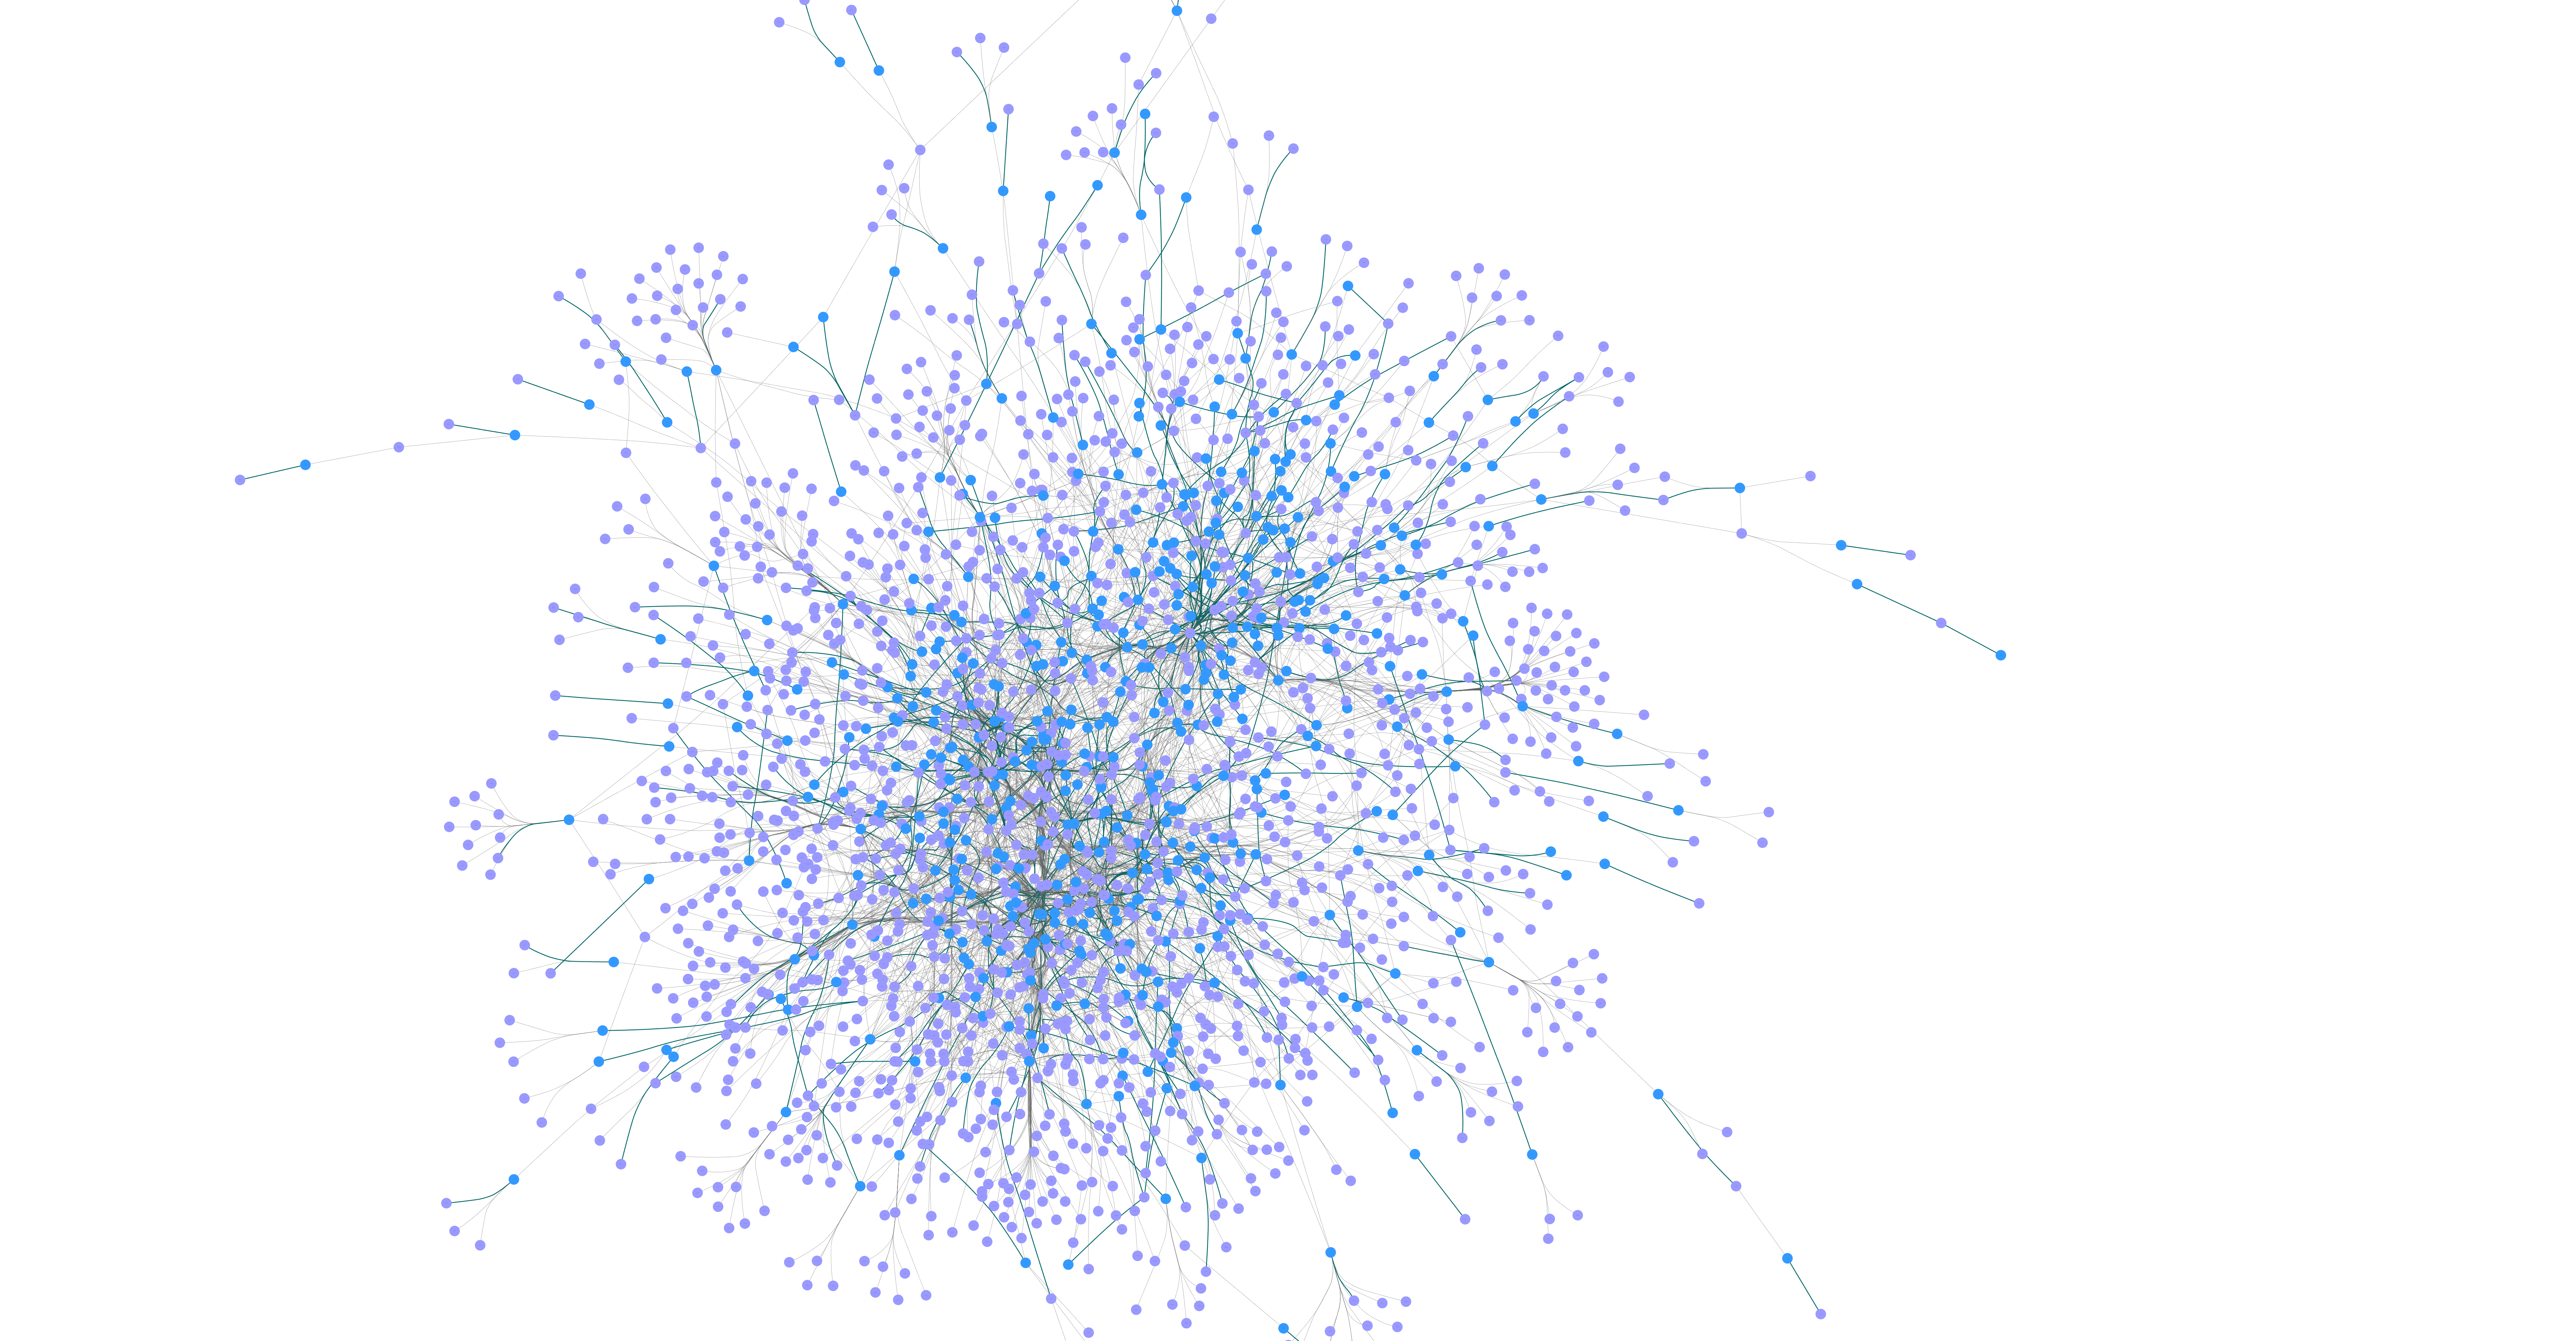
\includegraphics[width=0.5\textwidth]{Coraline_network.png}
    \caption{Network of Coraline fanfiction. Blue nodes represent stories, violet nodes represent users. Darker edges represent authorship, lighter edges represent a review.}
    \label{fig:coraline_network}
\end{figure}

\section{Related Work}

Within the last few years has there been an increase in large-scale computational analyses. \cite{milli2016beyond} compared fanfiction with the source (canon) text that stories originated from, performed sentiment analysis on the reviews, and predicted how readers would respond to characters in a chapter.

\cite{yin2017no} published an anonymized set of metadata, and presented evidence that the majority of users were English-speaking students based on the time of year FanFiction.Net users were most active.  This partially answered one of the questions posed by \cite{barnes2015fanfiction}, ``who writes fanfiction?"  While this meta-dataset may give valuable insight to many problems, it also eliminates one of the most valuable properties: the social network structure which exists between users and stories.

\section{Collaborative Filtering}

Document search is often performed as a combination of two components: \textit{content filtering} to find relevant keywords, document attributes, or metadata; and \textit{collaborative filtering} for evaluating relevancy through a popularity or similarity metric.

Collaborative filtering in networks or graph models may be performed in supervised or unsupervised manners for determining local, quasi-local, or global similarity \cite{nickel2016review,breese1998empirical}.

Unsupervised global similarity methods such as PageRank may provide insight to what is popular across all users in the a network, but may be less insightful when certain parts of the network are only relevant to certain users. Local similarity methods such as random walks may focus on parts of the network which are most relevant to certain users, but may not reach far enough outside of what the user is already aware of.

Supervised methods for collaborative filtering turn the previous into a learning problem where it is assumed that the similarity between two entities or relationships may be inferred from some observed properties of the data. These methods come with all of the difficulties of machine learning, such as balancing overfitting against generalization; but a prominent difficulty of these methods lies in the imbalance between the false positives and false negatives. A recommendation system that recommends everything to a user is not 

\cite{yang2017combining} recently

\section{Experiments}

The author poses and answers the following questions:

\begin{enumerate}
    \item[\textbf{Q1}:] How effective are the models at generalizing within and across communities when predicting story authorship?
    \item[\textbf{Q2}:] Does a greater number of facts in the training set directly lead to better results on the test set?
    \item[\textbf{Q3}:] Does soft margin improve performance over the default settings?
\end{enumerate}

\subsection{Creating a FanFiction Data Set}

All authors and stories on FanFiction.Net may be identified by a unique integer, which naturally lends itself to a relational representation. The meta-data about each story includes attributes such as the number of words, number of chapters, main characters, genres, and rating. Stories may be introduced with a summary in fewer than 384 characters, but these are not included here. Stories may be divided into chapters, and chapters may be reviewed by the author or other community members.

Four communities on the FanFiction.Net books category were selected for these experiments: \textit{Coraline}\footnote{https://www.fanfiction.net/book/Coraline/}, \textit{Hitchhiker's Guide to the Galaxy}\footnote{https://www.fanfiction.net/book/Hitchhiker-s-Guide-\\to-the-Galaxy/}, \textit{To Kill a Mockingbird}\footnote{https://www.fanfiction.net/book/To-Kill-a-Mockingbird/}, and \textit{Dragonriders of Pern series}\footnote{https://www.fanfiction.net/book/Dragonriders-of-Pern-series/}.

Data was scraped from these communities between April 24 and April 27, 2018, and four features were chosen to learn and make predictions about story authorship: \texttt{author} (the target attribute), \texttt{genre}, \texttt{rating}, and \texttt{reviewed}. \texttt{author} is a binary predicate distinguishing that a user wrote a story. \texttt{rating} is an attribute describing the fiction rating of a story \cite{fictionratings}. \texttt{genre} describes the genre of a story (Adventure, Horror, etc.), a story may have up to three genres but for simplicity all genres for a story are stored as a single value. \texttt{reviewed} is a binary predicate indicating that a particular user reviewed a particular story.  These features were chosen under the assumption that in these communities:

\begin{itemize}
    \item Authors are more likely to write stories with similar genres and ratings: an author tends not to write for all genres with equal frequency.
    \item Users tend to review stories with some genres or ratings as opposed to others, and personal preferences dictate what those may be.
    \item Users are more likely to review stories by the same author, either due to popularity of a story or an author's network of followers.
\end{itemize}

Though more features (such as word count, correlation metrics, review sentiment) may be vital for deeper insights, these four are appropriate to establish baselines and gain some insight to the prior assumptions.

% Coraline: Learn Negative: 160,873
% Coraline: Infer Negative: 29,215

% Hitchhikers: Learn Negative: 177,362
% Hitchhikers: Infer Negative: 32,322

% Dragonriders: Learn Negative: 174,607
% Dragonriders: Infer Negative: 31,833

% Mockingbird: Learn Negative: 190,051
% Mockingbird: Infer Negative: 34,563

%        Facts:
% Coraline    : 4,981
% Dragonriders: 6,678
% Hitchhikers : 5,240
% Mockingbird : 3,793

\begin{table}
\centering

    \begin{tabular}{|p{0.2\linewidth} p{0.13\linewidth}|p{0.03\linewidth} p{0.13\linewidth}|p{0.03\linewidth} p{0.13\linewidth}|}
    \hline
    & & \multicolumn{2}{|c|}{Learning} & \multicolumn{2}{|c|}{Inference} \\
    \hline
         Community & \# facts & pos & neg & pos & neg \\
         \hline
         Coraline & 4,981 & 402 & 160,873 & 173 & 29,215 \\
         Dragonriders & 6,678 & 421 & 174,607 & 179 & 31,833 \\
         Hitchhikers & 5,240 & 423 & 177,362 & 180 & 32,322 \\
         Mockingbird & 3,793 & 438 & 190,051 & 187 & 34,563 \\
    \hline
    \end{tabular}

    \caption{The number of positives, negatives, and facts for each community during learning and inference. For evaluation, \texttt{author} values were randomly assigned to a learning or inference set based on a 70\%/30\% train/test split, and these splits were sampled and averaged ten times.}
    \label{tab:data_overview}
\end{table}

These communities were selected because they shared a similar number of stories (between 575 and 625). Though the communities were similar by this metric, there was a prominent difference in the number of facts: \textit{To Kill a Mockingbird} had the highest number of stories, but the fewest facts; \textit{Dragonriders of Pern series} had the second-fewest number of stories, but a significantly more facts. This is because the number of facts associated with a community is heavily biased by the number of reviews across a community's stories. This may be a way to gain insight into community activity in subsequent studies.

\subsection{Learning and Inference with BoostSRL}

Facts were made available during both learning and inference whereas positive examples were assigned randomly to a learning or inference set to make predictions.  Negative examples were sampled under the closed-world assumption from the respective positive set, but because the number of negatives is determined from the positives: the number reported for each learning and inference set is an average from 100 samples.

The author employs a state-of-the-art statistical relational learning system: \textit{BoostSRL} to learn relational dependency networks over the features. Two methods are compared: boosted relational dependency networks (RDN-Boost), and boosted relational dependency networks with soft margin (Softm-Boost). For both methods, the learning and inference sets were sampled from master sets for each community, and precision/recall scores were calculated based on an average over ten independently sampled runs. To evaluate how general these models are, the learning and inference sets may be drawn from two different communities: learning may be done on a set of stories drawn from \textit{Coraline}, but inference may be performed on stories from the \textit{Hitchhiker's Guide to the Galaxy} community.

For both RDN-Boost and Softm-Boost, all settings were kept constant, including: tree depth, node size, mode settings, and number of regression trees learned during training (15). The only exception was the use of soft margin with false negative ($\alpha$) weight of 0 and a false positive ($\beta$) weight of 2 in order to increase the cost of returning false positives.

\cite{yang2017combining} used similar settings to these and claimed that learning more than 20 trees had little affect on overall performance. Varying these settings with careful tuning may lead to better performance, but is not explored within the context of this paper.

\section{Results}

% Q1) How effective are the models at generalizing within and across communities when predicting story authorship?
% Q2) Does a greater number of facts in the training set directly lead to better results on the test set?
% Q3) Does soft margin improve performance over the default settings?

Table \ref{tab:results} displays the results of the experiments. Soft margin leads to a massive improvement in recall across all training and test splits, but precision appears to be negatively affected in some cases. \textbf{Q3} may be accepted in this case: if the goal is high recall, then the soft margin approach should at least be explored.

If the number of facts available during learning lead to better results on the given test set, it would generally be assumed that the set with the most facts would lead to the best performance while the set with the fewest facts would lead to generally less-good performance. In this case, \textit{Dragonriders of Pern series} had the highest number of facts (6,678) while \textit{To Kill a Mockingbird} had the fewest (3,793). For both RDN-Boost and Sofm-Boost, the best performance tends not to be based on the number of facts available during learning or inference, but whether learning and inference draws examples from the same community. This provides insight to answering both \textbf{Q1} and \textbf{Q2}: more data does not necessarily imply better results when the underlying data is drawn from different distributions; but the performance does not drop in such a catastrophic manner to make us assume that generalization does not occur at all.

% Tables are quite large, it will likely be easier if they extend across both columns.
% https://texblog.org/2012/07/30/single-column-figuretable-in-a-two-multi-column-environment/
\begin{table*}[ht]
\centering

        % Table 1: RDN-Boost Precision
        \begin{tabular}{|p{0.15\linewidth}|p{0.15\linewidth}|p{0.15\linewidth}|p{0.15\linewidth}|p{0.15\linewidth}|}
        \hline
        \multicolumn{5}{|c|}{RDN-Boost Precision}\\
        \hline
            & Coraline & Dragonriders & Hitchhikers & Mockingbird \\
            \hline
             Coraline & \textbf{0.014} & \textbf{0.009} & 0.013 & 0.012 \\
             Dragonriders & 0.008 & \textbf{0.009} & 0.009 & 0.013 \\
             Hitchhikers & 0.013 & 0.008 & \textbf{0.019} & 0.014 \\
             Mockingbird & \textbf{0.014} & 0.007 & 0.013 & \textbf{0.034} \\
        \hline
        \end{tabular}
        
        % Table 2: RDN-Boost Recall
        \begin{tabular}{|p{0.15\linewidth}|p{0.15\linewidth}|p{0.15\linewidth}|p{0.15\linewidth}|p{0.15\linewidth}|}
        \hline
        \multicolumn{5}{|c|}{RDN-Boost Recall}\\
        \hline
            & Coraline & Dragonriders & Hitchhikers & Mockingbird\\
            \hline
            Coraline & 0.119 & 0.092 & 0.062 & 0.065 \\
            Dragonriders & 0.037 & 0.083 & 0.063 & 0.050 \\
            Hitchhikers & 0.206 & 0.227 & 0.193 & 0.075 \\
            Mockingbird & 0.331 & 0.415 & 0.258 & 0.210 \\
        \hline
        \end{tabular}
        
        % Table 3: Softm-Boost Precision
        \begin{tabular}{|p{0.15\linewidth}|p{0.15\linewidth}|p{0.15\linewidth}|p{0.15\linewidth}|p{0.15\linewidth}|}
        \hline
        \multicolumn{5}{|c|}{Softm-Boost Precision}\\
        \hline
            & Coraline & Dragonriders & Hitchhikers & Mockingbird \\
            \hline
             Coraline & \textbf{0.014} & \textbf{0.011} & 0.013 & 0.001 \\
             Dragonriders & 0.009 & 0.010 & 0.008 & 0.008 \\
             Hitchhikers & 0.010 & 0.008 & \textbf{0.023} & 0.016 \\
             Mockingbird & 0.009 & 0.008 & 0.015 & \textbf{0.025} \\
        \hline
        \end{tabular}
        
        % Table 4: Softm-Boost Recall
        \begin{tabular}{|p{0.15\linewidth}|p{0.15\linewidth}|p{0.15\linewidth}|p{0.15\linewidth}|p{0.15\linewidth}|}
        \hline
        \multicolumn{5}{|c|}{Softm-Boost Recall}\\
        \hline
            & Coraline & Dragonriders & Hitchhikers & Mockingbird \\
            \hline
             Coraline & 1.0 & 1.0 & 1.0 & 1.0 \\
             Dragonriders & 1.0 & 1.0 & 1.0 & 1.0 \\
             Hitchhikers & 1.0 & 1.0 & 1.0 & 1.0 \\
             Mockingbird & 1.0 & 1.0 & 1.0 & 1.0 \\
        \hline
        \end{tabular}

    \caption{Precision and recall values for RDN-Boost and Softm-Boost. Rows represent the learning set, columns represent the inference set. Precision values are highlighted if they are the highest in either a row or column.}
    \label{tab:results}

\end{table*}

\section{Conclusion}

These results are still fairly early in the process toward something which could become a collaborative filtering engine for FanFiction.Net, or a full paper extending what is known about several communities on FanFiction.Net. The evaluation criteria presented here were measured against what is an extremely difficult task of predicting authorship from a small number of features. In addition to the open problems left over from these results, some of the key takeaway messages should be these: (1) FanFiction.Net has rich social network properties which should be further explored within the statistical relational learning community, and the computer science community more broadly. (2) FanFiction.Net is the embodiment of a time-evolving social network, where people who share common interests read, write, and review stories.

\section{Appendix}

\subsection{Scraping FanFiction.Net}

The terms of service for FanFiction.Net state the limitations of launching automated bots in Section 4, Paragraph E of their terms of service\footnote{https://www.fanfiction.net/tos/}, paraphrased here:

\begin{itemize}
    \item ``You agree not to use or launch any automated system... that accesses the Website in a manner that sends more request messages... than a human can reasonably produce in the same period....''
    \item ``FanFiction.Net grants the operators of public search engines permission to use spiders... solely to the extent necessary for creating publicly available searchable indices... but not caches or archives....''
    \item ``You agree not to collect or harvest any personally identifiable information... for any commercial solicitation purposes.''
\end{itemize}

Scraping FanFiction.Net may be accomplished via the \texttt{ffscraper/} Python package in this repository. The core documentation pertaining to each script and their respective functions are contained therein, this discussion pertains to the high-level idea of what they accomplish.

All users and stories on FanFiction.Net may be identified via a unique id-number. These id-numbers may be used to directly access one or the other, for example: user \textit{124}'s profile may be found by sending a request to https://www.fanfiction.net/u/124. In a similar manner, story \textit{124} would be at https://www.fanfiction.net/s/124. Reviews for a story follow the pattern \texttt{/r/125/0/1/}, where the first integer corresponds the story-id, the second integer to a certain chapter (or 0 for all reviews), and the third is a page number (a maximum of 15 reviews are displayed on each page, so any overflow will be on subsequent pages).

\bibliographystyle{aaai}
\bibliography{link-prediction-fanfiction}

\end{document}
